\section*{1/18. feladat: Hasáb alakú tartály}
\addcontentsline{toc}{section}{1/18. feladat: Hasáb alakú tartály}
\begin{tabular}{ | p{2cm} | p{14cm} | } 
	\hline 
	Szerző & Cseresznyés Hunor, BO98IB \\
	\hline
	Szak & Biomérnök Bsc. \\
	\hline	Félév & 2019/2020 II. (tavaszi) félév  \\
	\hline
\end{tabular}
\vspace{0.5cm}

%========Feladat megfogalmazása=============
\noindent Egy négyzetes hasáb alakú tartály alapéle a= 60 cm, oldaléle l=2 m , ha $\rho= 1250  kg/m^3$ sűrűségű folyadékkal teletöltjük, mekkora az alaplapjára és az oldalfalára ható erő? $(g=9,81 m/s^2)$

%======Ábra============
\begin{figure}[h]
\centering
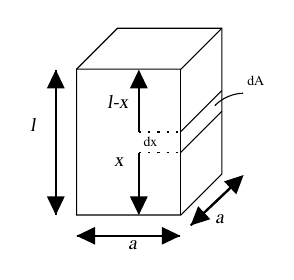
\begin{tikzpicture}[x=0.75pt,y=0.75pt,yscale=-1,xscale=1]


%=====Vonal ábrázolás=======
\draw   (310,39.72) -- (329.72,20) -- (380,20) -- (380,90.28) -- (360.28,110) -- (310,110) -- cycle ; \draw   (380,20) -- (360.28,39.72) -- (310,39.72) ; \draw   (360.28,39.72) -- (360.28,110) ;

\draw [line width=0.75]    (310,120) -- (357,120) ;
\draw [shift={(360,120)}, rotate = 180] [fill={rgb, 255:red, 0; green, 0; blue, 0 }  ][line width=0.08]  [draw opacity=0] (8.93,-4.29) -- (0,0) -- (8.93,4.29) -- cycle    ;
 
\draw [line width=0.75]    (300,110) -- (300,43) ;
\draw [shift={(300,40)}, rotate = 450] [fill={rgb, 255:red, 0; green, 0; blue, 0 }  ][line width=0.08]  [draw opacity=0] (8.93,-4.29) -- (0,0) -- (8.93,4.29) -- cycle    ;
 
\draw [line width=0.75]    (365,115) -- (388.3,92.8) ;
\draw [shift={(390.48,90.74)}, rotate = 496.4] [fill={rgb, 255:red, 0; green, 0; blue, 0 }  ][line width=0.08]  [draw opacity=0] (8.93,-4.29) -- (0,0) -- (8.93,4.29) -- cycle    ;
 
\draw [line width=0.75]    (385.48,95.74) -- (367.19,112.94) ;
\draw [shift={(365,115)}, rotate = 316.75] [fill={rgb, 255:red, 0; green, 0; blue, 0 }  ][line width=0.08]  [draw opacity=0] (8.93,-4.29) -- (0,0) -- (8.93,4.29) -- cycle    ;
 
\draw [line width=0.75]    (360,120) -- (313,120) ;
\draw [shift={(310,120)}, rotate = 360] [fill={rgb, 255:red, 0; green, 0; blue, 0 }  ][line width=0.08]  [draw opacity=0] (8.93,-4.29) -- (0,0) -- (8.93,4.29) -- cycle    ;
 
\draw [line width=0.75]    (300,40) -- (300,107) ;
\draw [shift={(300,110)}, rotate = 270] [fill={rgb, 255:red, 0; green, 0; blue, 0 }  ][line width=0.08]  [draw opacity=0] (8.93,-4.29) -- (0,0) -- (8.93,4.29) -- cycle    ;
 
\draw    (360,70) -- (380,50) ;
 
\draw    (360,80) -- (380,60) ;
 
\draw  [dash pattern={on 0.84pt off 2.51pt}]  (340,70) -- (360,70) ;

\draw  [dash pattern={on 0.84pt off 2.51pt}]  (340,80) -- (360,80) ;
 
\draw [line width=0.75]    (340,80) -- (340,107) ;
\draw [shift={(340,110)}, rotate = 270] [fill={rgb, 255:red, 0; green, 0; blue, 0 }  ][line width=0.08]  [draw opacity=0] (8.93,-4.29) -- (0,0) -- (8.93,4.29) -- cycle    ;

\draw [line width=0.75]    (340,70) -- (340,43) ;
\draw [shift={(340,40)}, rotate = 450] [fill={rgb, 255:red, 0; green, 0; blue, 0 }  ][line width=0.08]  [draw opacity=0] (8.93,-4.29) -- (0,0) -- (8.93,4.29) -- cycle    ;
 
\draw  [draw opacity=0] (376.63,57.28) .. controls (378.26,55.56) and (380.39,54.06) .. (382.9,52.97) .. controls (385.38,51.89) and (387.92,51.35) .. (390.28,51.32) -- (387.07,62.56) -- cycle ; \draw   (376.63,57.28) .. controls (378.26,55.56) and (380.39,54.06) .. (382.9,52.97) .. controls (385.38,51.89) and (387.92,51.35) .. (390.28,51.32) ;

%======Felirat=========
\draw (287.65,62) node [anchor=north west][inner sep=0.75pt]  [xslant=0.17] [align=left] {{\fontfamily{ptm}\selectfont {\scriptsize l}}};

\draw (334.72,121) node [anchor=north west][inner sep=0.75pt]  [xslant=0.2] [align=left] {{\fontfamily{ptm}\selectfont {\scriptsize a}}};

\draw (376.65,108.37) node [anchor=north west][inner sep=0.75pt]  [xslant=0.2] [align=left] {{\fontfamily{ptm}\selectfont {\scriptsize a}}};

\draw (324.69,51) node [anchor=north west][inner sep=0.75pt]  [xslant=0.16] [align=left] {{\fontfamily{ptm}\selectfont {\scriptsize l-x}}};

\draw (327.69,81) node [anchor=north west][inner sep=0.75pt]  [xslant=0.16] [align=left] {{\fontfamily{ptm}\selectfont {\scriptsize x}}};

\draw (341,71) node [anchor=north west][inner sep=0.75pt]   [align=left] {{\fontfamily{ptm}\selectfont {\tiny dx}}};

\draw (391,42) node [anchor=north west][inner sep=0.75pt]   [align=left] {{\tiny {\fontfamily{ptm}\selectfont dA}}};

\end{tikzpicture}
\end{figure}
%=====Feladat megoldása========

\noindent\hrulefill
\subsubsection{Feladat megoldás}
\noindent A nyomóerő merőlegesen hat a négyzet alakú hasáb alapjára. Ennek nagysága a nyomás és a felület nagyságának szorzatától függ. Az alapra irányuló nyomást meghatározhatjuk a folyadék sűrűségéből, a ránehezedő folyadékmagasság illetve a nehézségi erő szorzatából. Emellett definiálunk egy "A" felületelemet, aminek területe $a\cdot{a}$ lesz. Mértékegységekre figyeljünk!
\begin{equation}
F_a = p\cdot{A}=\rho\cdot{g}\cdot{l}\cdot{A}=8829 N
\end{equation}
\noindent{Tehát az alaplapjára ható erő: $\underline{\underline{8829 N}}$}

\vspace{0.5cm}

\noindent Az oldalfalára ható erő megállapításkor először válasszunk ki egy felületelemet (dA)-t és menjünk le differenciális szintre, erre a felületelemre vizsgáljuk meg a erőviszonyokat.Ha differenciális szinten eredményre jutunk, akkor terjesszük ki az egész felületelemre. Nézzük az egyenletek szempontjából:

\begin{equation}
dA= a\cdot{dx} 
\end{equation}

\begin{equation}
dF= p(x)\cdot{dA}
\end{equation}

\begin{equation}
p(x)= \rho\cdot{g}\cdot{(l-x)}
\end{equation}

\begin{equation}
\int dF =\int\rho\cdot{g}\cdot{(l-x)}\cdot{a}\cdot{dx}
\end{equation}

\begin{equation}
F =\rho\cdot{g}\cdot{a}\int_{0}^l(l-x)\cdot{dx}
\end{equation}

\begin{equation}
F =\rho\cdot{g}\cdot{a}\cdot[-\cdot(\frac{l-x}{2})^2]_{0}^l =\rho\cdot{g}\cdot{a}\cdot\frac{l^2}{2}=14715N
\end{equation}

\noindent {Tehát az oldalfalára ható erő: $\underline{\underline{14715 N}}$}

\vspace{0.5cm}
